\begin{frame}[c]{}

\centering
\huge
Lectures 9+10:\\
Meta-Learning I+II
\end{frame}
%----------------------------------------------------------------------
\begin{frame}[c]{Where are we? The big picture}

\begin{itemize}
	\item Introduction
	\item Background
	\begin{itemize}
		\item Design spaces in ML
		\item Evaluation and visualization
	\end{itemize}
	\item Hyperparameter optimization (HPO)
	\begin{itemize}
		\item Bayesian optimization
		\item Other black-box techniques
		\item More details on Gaussian processes
	\end{itemize}
	\item Pentecost (Holiday) -- no lecture
	\item Architecture search I + II
	\item[$\to$] Meta-Learning I + II
	\item Beyond AutoML: algorithm configuration and control
	\item Project announcement and closing
\end{itemize}

\end{frame}
%----------------------------------------------------------------------

%----------------------------------------------------------------------
\begin{frame}[c]{Learning Goals}

After these two lectures, you will be able to \ldots

\begin{itemize}
	\item explain the \alert{high-level principles of meta-learning} and its facets
	\item use \alert{algorithm selection} to predict the best algorithm for a dataset
	\item improve the performance of AutoML tools by \alert{warmstarting its search}
	\item \alert{transfer knowledge} between DNNs by determining initial weights
	\item \alert{learn} a DNN which can \alert{train} another DNNs
	\item \alert{learn} a policy \alert{to optimize} a black-box function
	\item \alert{learn} policies to either \alert{replace} algorithm components\\ or to \alert{control} hyperparameters
\end{itemize}

\pause
\medskip
\alert{Warning:} I gave my best to \alert{unify the notation} of different papers here. Please keep that in mind if you read the original papers which use different notations.

\end{frame}
%-----------------------------------------------------------------------
%----------------------------------------------------------------------
\begin{frame}[c]{Further Material}

There were two great tutorials on meta-learning recently:

\begin{itemize}
	\item NeurIPS'18: Frank Hutter and Joaquin Vanschoren
	"Automatic Machine Learning (AutoML): A Tutorial"
	\footnotesize{\url{https://videoken.com/embed/5A4xbv5nd8c}}
	\item ICML'19: Chelsea Finn and Sergey Levine on\\
	"Meta-Learning: from Few-Short Learning to Rapid Reinforcement Learning"\\
	\footnotesize{\url{https://www.facebook.com/icml.imls/videos/400619163874853/}}
\end{itemize}

\begin{itemize}
	\item We can't cover all the stuff in details
	\item Strong recommendation to watch both tutorials
	\item Parts of the material used today was inspired by these tutorials
\end{itemize}


\end{frame}
%-----------------------------------------------------------------------
\section{Meta-Learning}
%----------------------------------------------------------------------
\begin{frame}[c]{The Idea of Meta-Learning}

\begin{itemize}
	\item Learning essentially never stops
	\begin{itemize}
		\item We learn several models on the same task (e.g., dataset)
		\item We learn models on new tasks
	\end{itemize}
    \pause
    \item Learning is often done from scratch
    \item[$\leadsto$] We humans don't start from scratch all the time,\\
    but we learned how to learn!
\end{itemize}

\bigskip

\begin{tikzpicture}

	\node (task1) [data, text width=6em] {Task~1};
	\node (learn1) [activity, below of=task1, text width=6em] {Learning};
	\node (models1) [data, below of=learn1, text width=6em] {Models};
	\node (perf1) [data, below of=models1, text width=6em] {Performance};
	
	\node (task2) [data, right of=task1, node distance=4.5cm, text width=6em] {Task~2};
	\node (learn2) [activity, below of=task2, text width=6em] {Learning};
	\node (models2) [data, below of=learn2, text width=6em] {Models};
	\node (perf2) [data, below of=models2, text width=6em] {Performance};
	
	\node (task3) [data, right of=task2, node distance=4.5cm, text width=6em] {Task~3};
	\node (learn3) [activity, below of=task3, text width=6em] {Learning};
	\node (models3) [data, below of=learn3, text width=6em] {Models};
	\node (perf3) [data, below of=models3, text width=6em] {Performance};
	
	\draw[myarrow] (task1) -- (learn1);
	\draw[myarrow] (learn1) -- (task1);
	\draw[myarrow] (learn1) -- (models1);
	\draw[myarrow] (models1) -- (perf1);
	
	\draw[myarrow] (task2) -- (learn2);
	\draw[myarrow] (learn2) -- (task2);
	\draw[myarrow] (learn2) -- (models2);
	\draw[myarrow] (models2) -- (perf2);
	
	\draw[myarrow] (task3) -- (learn3);
	\draw[myarrow] (learn3) -- (task3);
	\draw[myarrow] (learn3) -- (models3);
	\draw[myarrow] (models3) -- (perf3);
	
	\pause
	
	\draw[myarrow, dashed] (learn1) -- node[above] {\alert{Meta-Learn}} (learn2);
	\draw[myarrow, dashed] (learn2) -- node[above] {\alert{Meta-Learn}} (learn3);	
	
	\pause
	\draw[myarrow, dashed] (models1) -- node[above] {\alert{Meta-Learn}} (models2);
	\draw[myarrow, dashed] (models2) -- node[above] {\alert{Meta-Learn}} (models3);
	
	\pause
	\draw[myarrow, dashed] (perf1) -- node[above] {\alert{Meta-Learn}} (perf2);
	\draw[myarrow, dashed] (perf2) -- node[above] {\alert{Meta-Learn}} (perf3);
\end{tikzpicture}

\end{frame}
%-----------------------------------------------------------------------
\begin{frame}[c]{Example for Human Meta-Learning}

\begin{columns}
	\column{0.18\textwidth}
	Braque
	\centering
	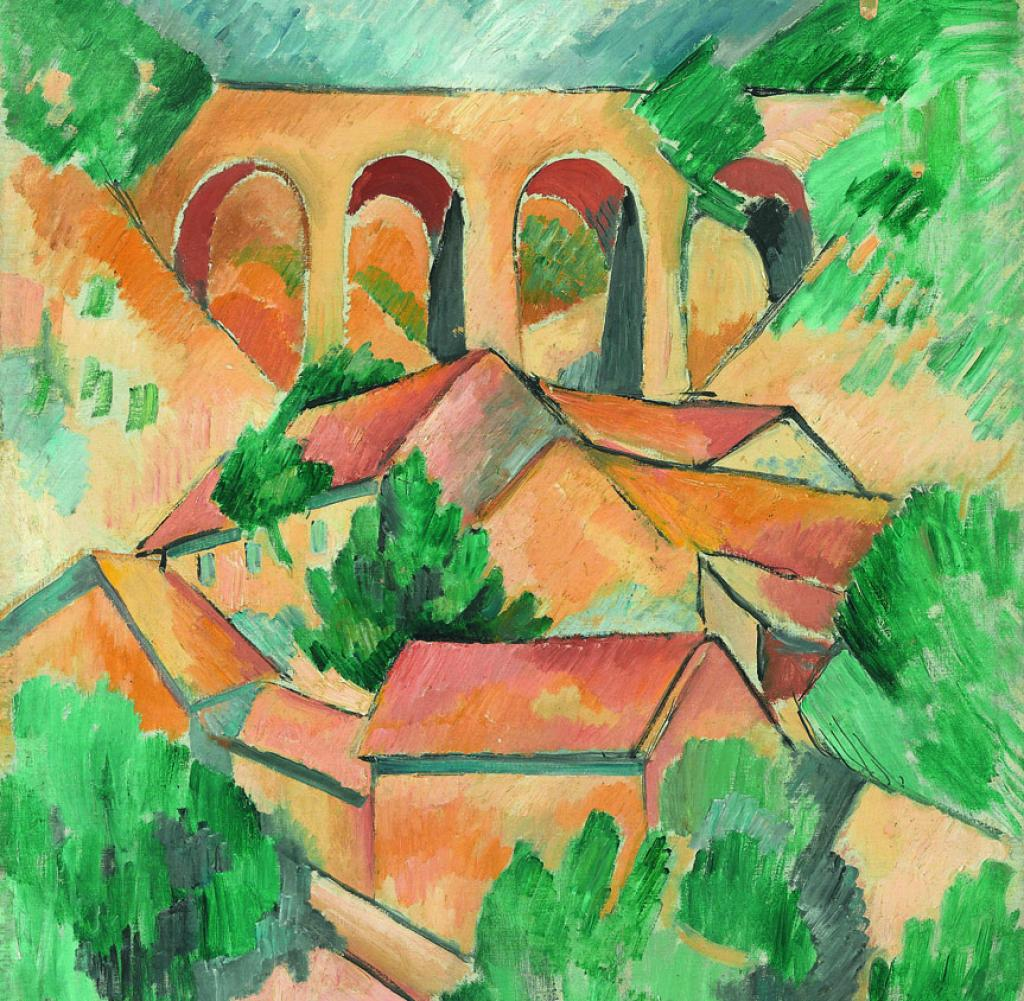
\includegraphics[width=1.0\textwidth]{images/braque1.jpg}
	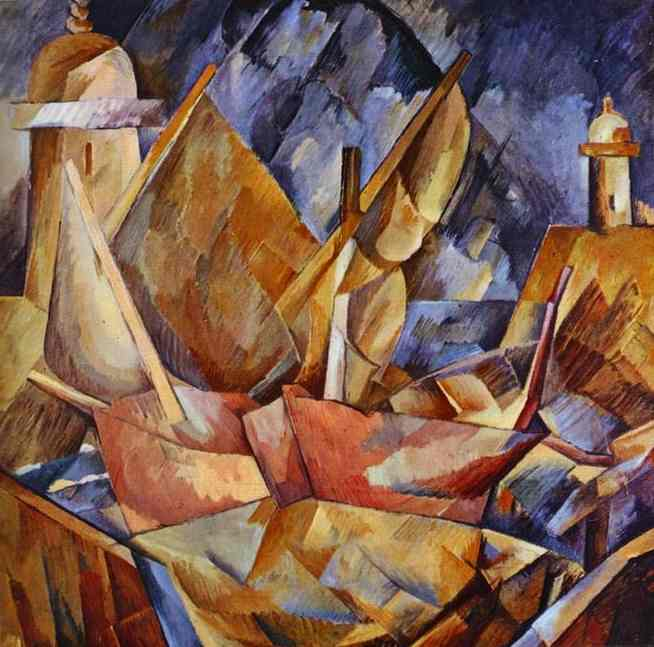
\includegraphics[width=1.0\textwidth]{images/braque2.jpeg}
	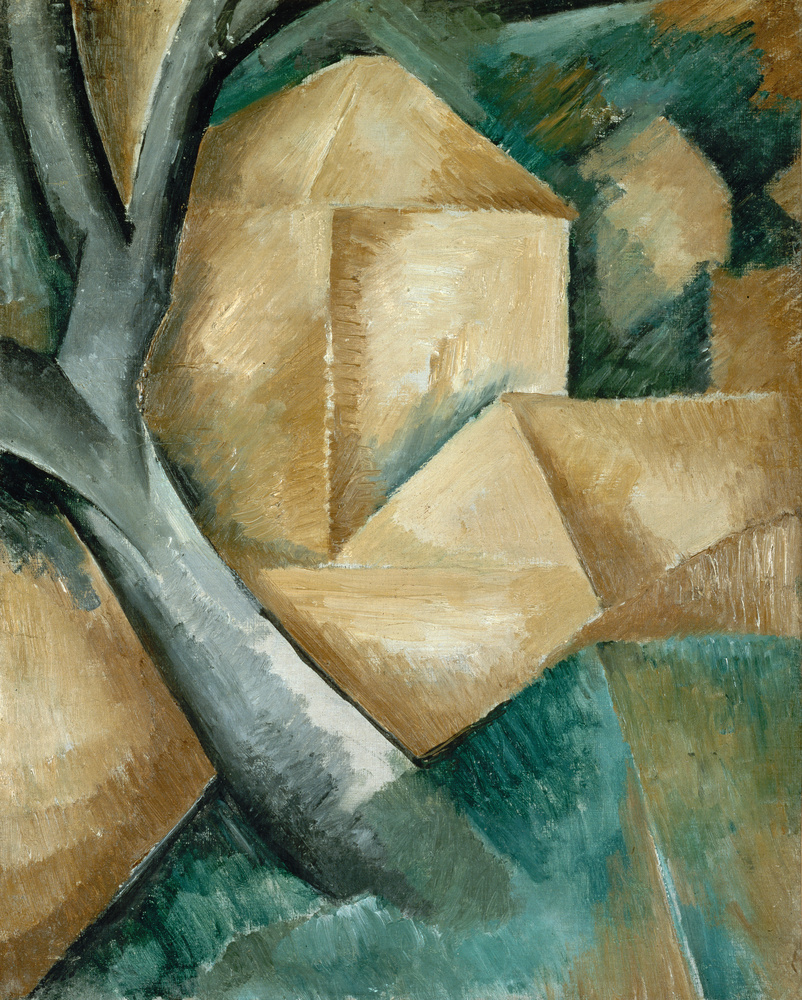
\includegraphics[width=1.0\textwidth]{images/braque3.jpg}
	\column{0.258\textwidth}
	Cezanne
	\centering
	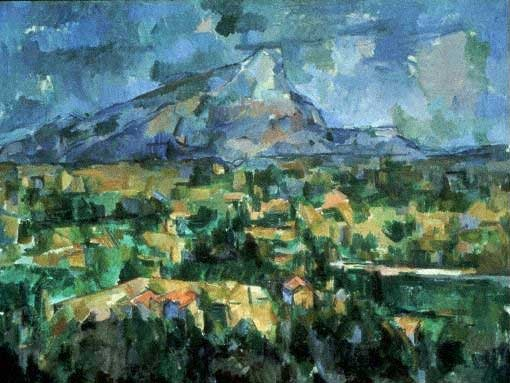
\includegraphics[width=1.0\textwidth]{images/cezanne1.jpg}
	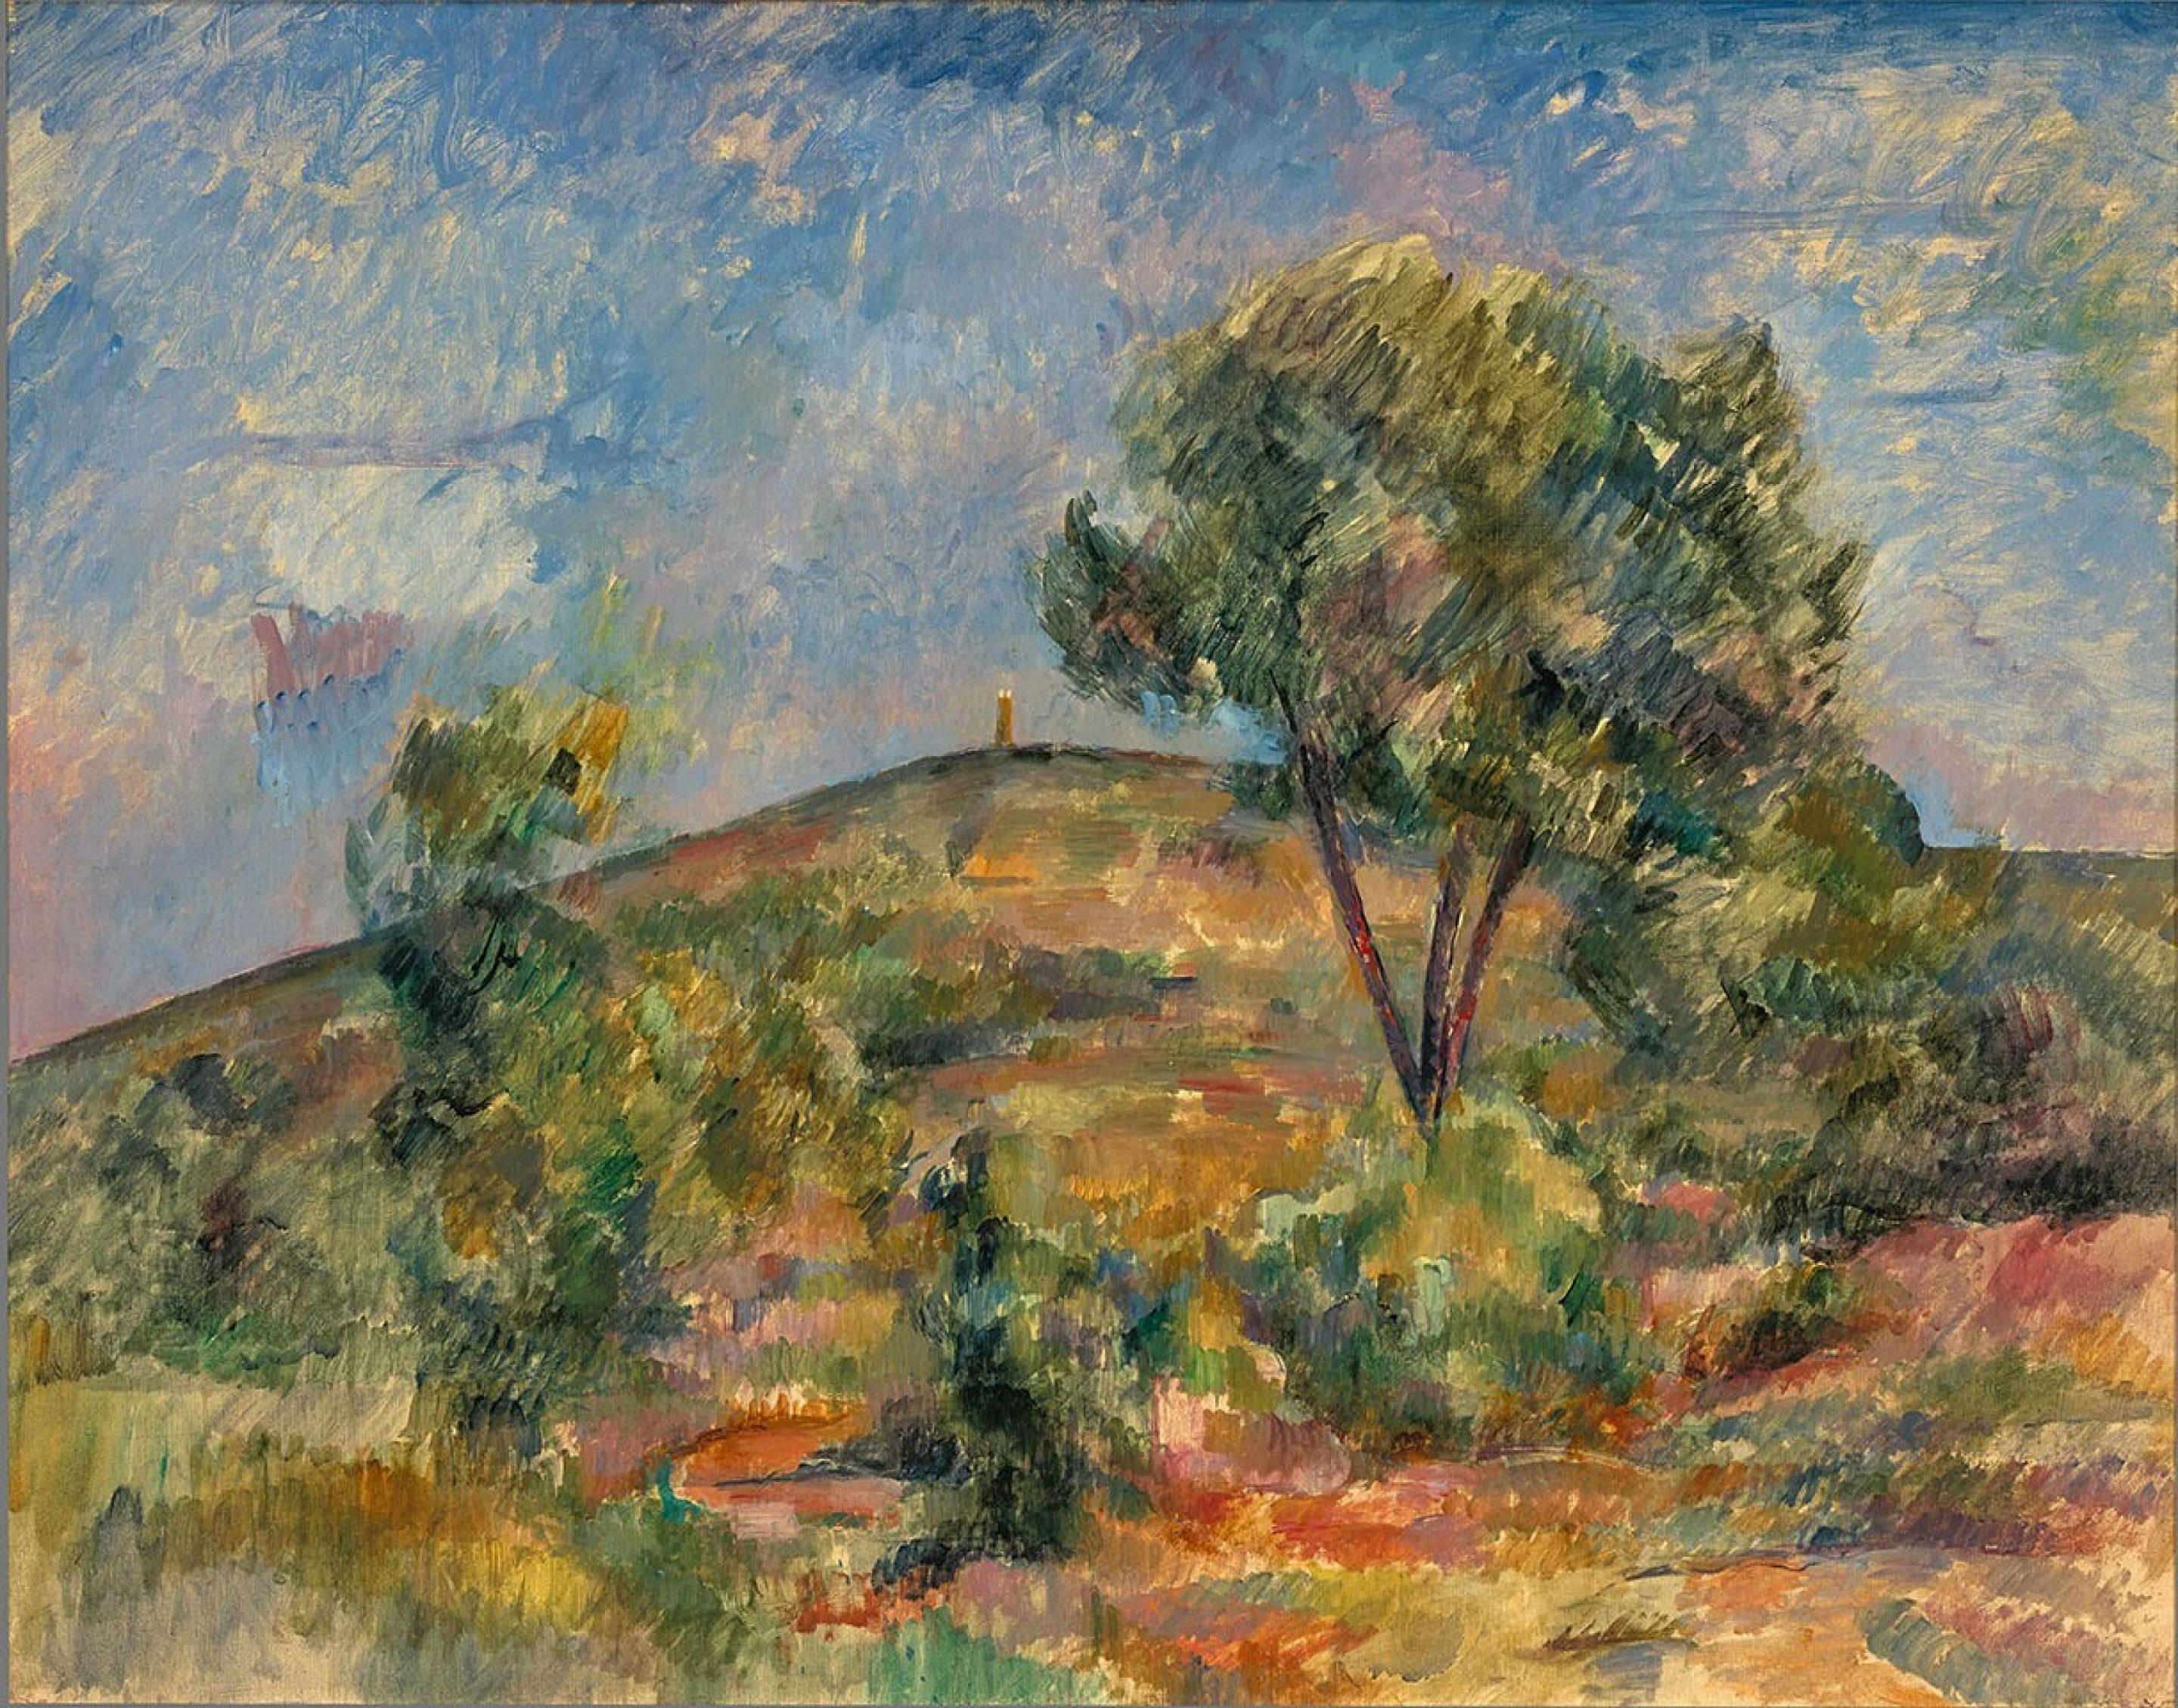
\includegraphics[width=1.0\textwidth]{images/cezanne2.jpg}
	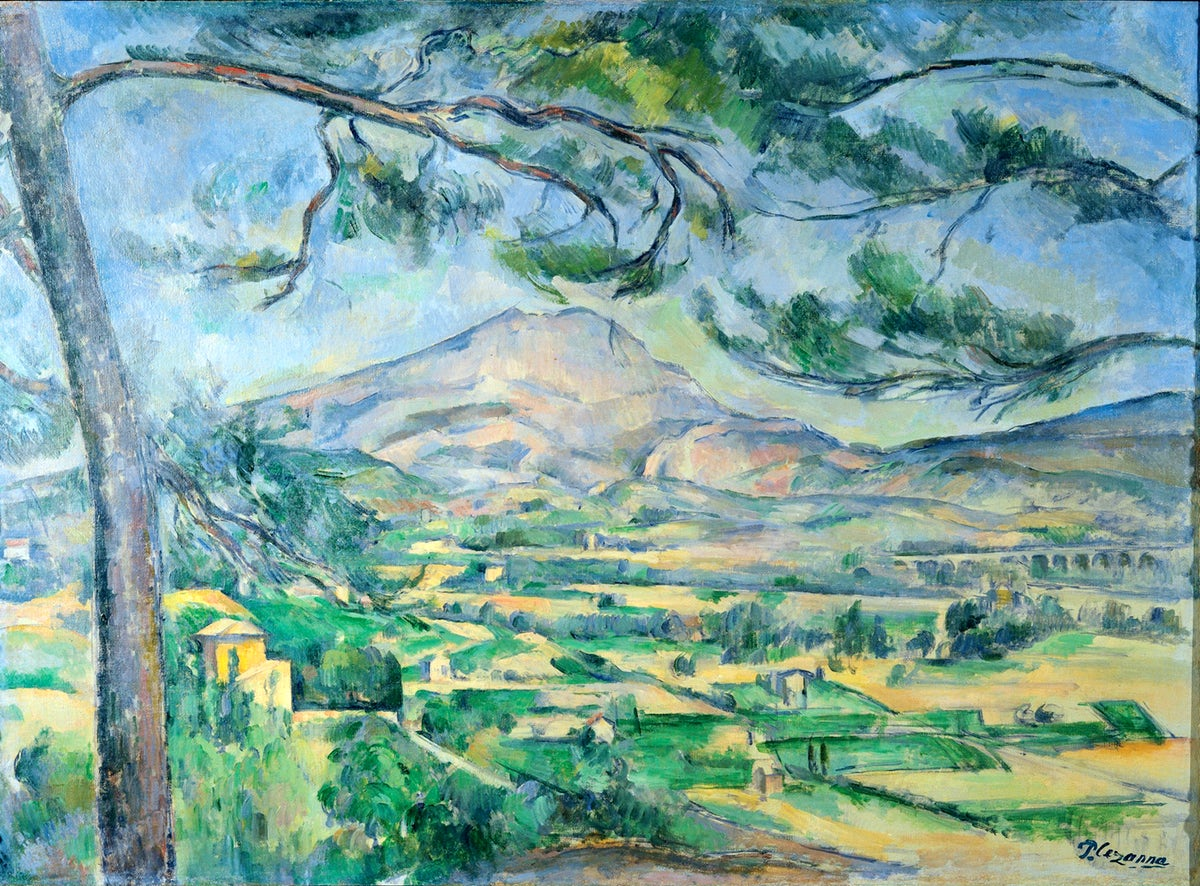
\includegraphics[width=1.0\textwidth]{images/cezanne3.jpg}
	\column{0.3\textwidth}
	\centering
	Who painted that?
	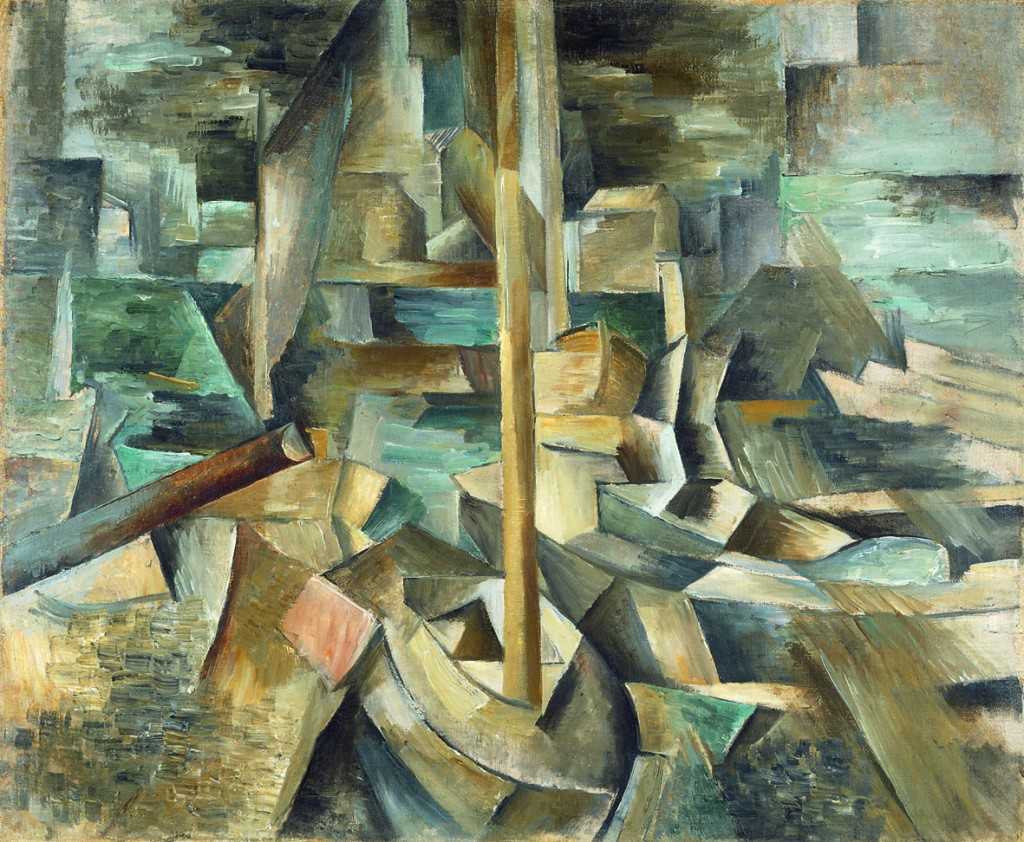
\includegraphics[width=1.0\textwidth]{images/Braque4.jpg}
	
	\pause
	Most likely most of you can identify the painter correctly, 
	although I presented only three pictures of each.
\end{columns}

\end{frame}
%-----------------------------------------------------------------------
%-----------------------------------------------------------------------
\begin{frame}[c]{Recap Supervised Learning}

Dataset:
\begin{equation}
\dataset = \{(x_1, y_1), \ldots, (x_k, y_k) \}
\end{equation}

\bigskip
\pause

Learning a model $\phi$ (e.g., weights of a neural network):
\begin{eqnarray}
\argmax_{\phi} \log p(\phi|\dataset)\\
\pause
= \argmax_{\phi} \log p(\dataset | \phi) + \log p(\phi) \\
\pause
= \argmax_{\phi} \sum_i \log p(y_i | x_i, \phi) + \log p(\phi)
\end{eqnarray}

\pause

Challenge:
\begin{itemize}
	\item Learning starts from scratch\\
	(e.g., we initially have no clue how to learn a good $\phi$)
	\item we might only have very few examples in $\dataset$ 
	(i.e., $k$ is small)
\end{itemize}

\end{frame}
%-----------------------------------------------------------------------
%-----------------------------------------------------------------------
\begin{frame}[c]{The Meta Learning Problem}

Dataset:
\begin{equation}
\dataset = \{(x_1, y_1), \ldots, (x_k, y_k) \}
\end{equation}
Set of datasets (meta-datasets):
\begin{equation}
\mdata = \{\mathcal{D}_1, \ldots, \mathcal{D}_n, \}
\end{equation}

\pause
Can we include these meta-datasets to improve learning on $\dataset$?
\begin{equation}
\argmax_{\phi} \log p(\phi|\dataset, \mdata)
\end{equation}

\pause
\medskip

\alert{Idea:} Instead of keeping $\mdata$ forever, we want to distill the knowledge into \alert{meta-parameters $\theta$}: $p(\theta|\mdata)$
 

\end{frame}
%-----------------------------------------------------------------------
%-----------------------------------------------------------------------
\begin{frame}[c]{The Meta Learning Problem}

In meta-learning, we want to learn:
\begin{eqnarray}
\argmax_{\phi} \log p(\phi|\dataset, \mdata) \\
\pause
= \argmax_{\phi} \log \int_{\Theta} p(\phi \mid \dataset, \theta) p(\theta \mid \mdata) d\theta\\
\pause
\approx \argmax_{\phi} \log p(\phi | \dataset, \theta^*) + \log p(\theta^* | \mdata)\\
\pause
= \argmax_{\phi} \log p(\phi | \dataset, \theta^*)
\end{eqnarray}

\pause

The meta-learning problem is:
\begin{equation}
\theta^* \in \argmax_{\theta} \log p(\theta | \mdata)
\end{equation}


\end{frame}
%-----------------------------------------------------------------------
%-----------------------------------------------------------------------
\begin{frame}[c]{AutoML $\subset$ Meta-Learning}

\begin{itemize}
	\item AutoML can be seen as a special case of meta-learning
	\pause
	\medskip
	\item $\theta$ could be:
	\begin{itemize}
		\item a hyperparameter configuration ($\lambda$) 
		\item a neural network architecture
	\end{itemize}
	\pause
	\medskip
	\item What would be $\mdata$ here? \hands
	\pause
	\begin{itemize}
		\item the train and validation dataset?
		\item a dataset on which we optimized $\lambda$ (e.g., CIFAR-10)\\ such that we can use it on another dataset (e.g., imagenet)
	\end{itemize}
\end{itemize}	

\end{frame}
%-----------------------------------------------------------------------
%-----------------------------------------------------------------------
\begin{frame}[c]{Meta-Learning $\subset$ AutoML}

\begin{itemize}
	\item Meta-learning can be powerful to complement AutoML
	\pause
	\medskip
	\item We can learn a lot of things $\mdata$ to improve the performance on new datasets
	\begin{itemize}
		\item pre-initialization of networks weights\\
		(e.g., pre-train on imagenet and fine-tune on a new dataset)
		\item learning a meta-DNN to predict how to train another target-DNN\\
		(more next week)
	\end{itemize}
	\pause
	\medskip
	\item Open question: If we can learn how to learn,\\ do we need AutoML anymore?
\end{itemize}

\end{frame}
%-----------------------------------------------------------------------
%-----------------------------------------------------------------------
\section{Algorithm Selection}
%----------------------------------------------------------------------
\begin{frame}[c]{Idea: Algorithm Selection}

\begin{itemize}
	\item By applying ML to many different datasets,\\
	humans get an intuition \alert{what works well on which dataset}
	\pause
	\item E.g., humans came up with rule of thumbs:\\
	"On small datasets we use an SVM, on mid-size dataset a RF\\ 
	and on big data a DNN"
	\pause
	\item Although these rule thumbs are quite useful,
	they are often not correct and simplify real applications too strongly
	\pause
	\item \alert{Question}: Can we learn from data which algorithm we should use for a given dataset?
\end{itemize}


\end{frame}
%-----------------------------------------------------------------------
%----------------------------------------------------------------------
\begin{frame}[c]{Definition: Algorithm Selection \litw{Rice 1976}}

\begin{block}{Definition}
	Given 
	\begin{itemize}
		\item a \alert{distribution} $\mdata$ of meta datasets,
		\item a portfolio of algorithms $\algo \in \portfolio$,
		\item and a cost metric $c:  \portfolio \times \mdata \rightarrow \perf$,   
	\end{itemize}
	
	the \emph{per-instance algorithm selection problem} is to find a mapping 
	$s: \dataset \mapsto \algo$ 
	that optimizes 
	$$\argmin_{s} \int_{\mdata} c(s(\dataset),\dataset) p(\dataset)  d\dataset$$
\end{block}


\end{frame}
%-----------------------------------------------------------------------
%----------------------------------------------------------------------
\begin{frame}[c]{Meta-Features in Machine Learning}
	
To learn the mapping $s: \dataset \mapsto \algo$, we need a way to represent $\dataset$

\begin{center}
	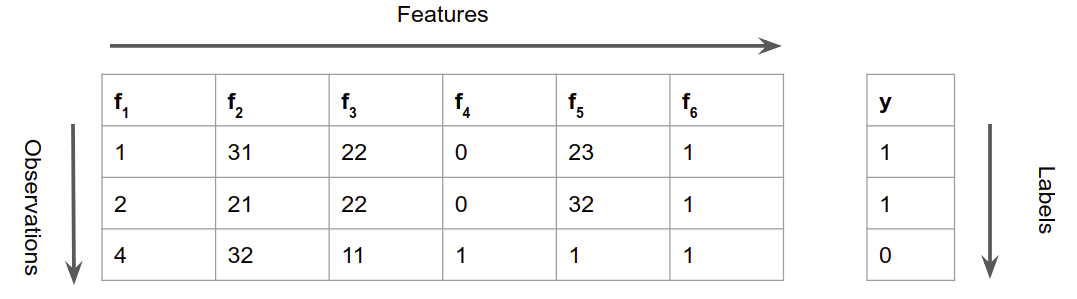
\includegraphics[width=0.7\textwidth]{images/ml_data}
\end{center}


What kind of ``Meta-features'' could describe a dataset? \hands

\pause
\begin{itemize}
	\item number of observations (samples)
	\item number of features
	\item number of classes
	\item number of categorical features
	\item number of numeric features
	\item percentage of numeric features
	\item number of missing features
	%\item number of observations belonging to most frequent class
	\item Probing: accuracy of a small decision tree
\end{itemize}
	
	
\end{frame}
%-----------------------------------------------------------------------
%----------------------------------------------------------------------
\begin{frame}[c]{Assumptions for Traditional Algorithm Selection}

We assume for a discrete set of datasets from $\mdata$ that
\begin{itemize}
	\item we have \alert{pre-computed meta-features} on all datasets
	\pause
	\begin{itemize}
		\item if our cost metric is not related to runtime,\\
		we assume that the cost for computing the meta features is\\ negligible compared to training a model
	\end{itemize}
	\pause
	\item we have measured the \alert{cost $c(\algo, \dataset)$} on all possible pairs $\langle \algo, \dataset\rangle$
\end{itemize}

\pause
\medskip

$\leadsto$ We have two matrices as training data,\\ one with meta-features and one with cost values

\end{frame}
%-----------------------------------------------------------------------
%----------------------------------------------------------------------
\begin{frame}[c]{Algorithm Selection as a Regression Problem}

\begin{itemize}
	\item Given a new dataset and its meta-features $f(\dataset)$
	\item we "only" need to predict the performance of all algorithms $\algo \in \portfolio$
	\item For each algorithm $\algo \in \portfolio$, we train a regression model to predict its cost $c(\algo,\dataset)$ given $\dataset$'s meta features:
	$$\hat{m}_\algo: f(\dataset) \mapsto c(\algo, \dataset) $$
	\pause
	\item Selection for given test $\dataset_{\text{test}}$:
	$$\argmin_{\algo \in \portfolio} \hat{m}_\algo(f(\dataset_{\text{test}}))$$
	\pause
	\item Remarks:
	\begin{itemize}
		\item As regression approach, we can essentially use whatever you want\\
		e.g., ridge regression, a random forest or a neural network
		\pause
		\item We could also train one joint model with indicator features for the algorithms
	\end{itemize}
\end{itemize}


\end{frame}
%-----------------------------------------------------------------------
%----------------------------------------------------------------------
\begin{frame}[c]{Algorithm Selection as a Classification Problem}

\begin{itemize}
	\item Learning a regression problem is an indirect approach solving the algorithm selection problem
	\pause
	\item Can we directly solve the multi-class classification problem?
	$$s: \dataset \mapsto \algo$$
	\pause
	\item We can use common approach for multi-class classification
	\pause
	\item Algorithm selection has a special characteristic:\\
	\alert{Some datasets are more sensitive to algorithm selection than others}
	\begin{itemize}
		\item for very easy datasets, it might not matter which algorithm to use
		\item for very hard datasets (e.g., because of poor data quality),\\ all algorithms might fail
		\item for all others, it might be important to select the right algorithm
	\end{itemize}
	
\end{itemize}


\end{frame}
%-----------------------------------------------------------------------
%----------------------------------------------------------------------
\begin{frame}[c]{Pairwise Cost-Sensitive Classification Problem \litw{Xu et al. 2011}}

\begin{itemize}
	\item The cost-sensitivity of a dataset $\dataset$ to algorithm selection across a portfolio is somehow hard to measure
	\pause
	\item For each pair of algorithms $\langle \algo_i, \algo_j \rangle$ we can easily measure the cost-sensitivity by
	$$sim(\dataset, \algo_i, \algo_j) = || c(\algo_i, \dataset) - c(\algo_j, \dataset) ||$$
	\pause
	\item Train for each pair of algorithms a classification model $s_{ \algo_i, \algo_j}$ predicting which algorithm performs better
	\pause
	\item consider for each training dataset $\dataset_{\text{train}}$ the $sim(\dataset_{\text{train}}, \algo_i, \algo_j)$
	\begin{itemize}
		\item cost-sensitive classification is often possible by modifying the loss function or split metric in tree-based approaches
	\end{itemize}
	\pause
	\item Selection for given test $\dataset_{\text{test}}$:
	$$\argmax_{\algo \in \portfolio} \sum_{\algo' \in \portfolio} s_{\algo, \algo'}(f(\dataset_{\text{test}})) $$
	
\end{itemize}

\end{frame}
%-----------------------------------------------------------------------
%----------------------------------------------------------------------
\begin{frame}[c]{Remarks on Algorithm Selection}

\begin{itemize}
	\item Pairwise cost-sensitive classification requires $\sim |\portfolio|^2 / 2$ models
	\pause
	\item From our experience, pairwise cost-sensitive approaches often perform better than regression approaches, but not always
	\pause
	\item We use machine learning to optimize machine learning
	\begin{itemize}
		\item Also the meta learning level can benefit from AutoML\\ \lit{Lindauer et al. 2015}
	\end{itemize}
	\pause
	\item Algorithm selection is not limited to machine learning
	\item Algorithm selection can be applied to any application where 
	\begin{enumerate}
		\pause
		\item we have a discrete portfolio of algorithms to choose from
		\pause
		\item the tasks (a.k.a. datasets) are sensitive to the algorithm choice\\ (so called heterogeneous tasks/instances)
		\pause
		\item we have informative meta-features (a.k.a. instance features)\\
		(only partially true for ML)
	\end{enumerate}
	\pause
	\item There is a benchmark library for algorithm selection data called ASlib (\url{www.aslib.net}) \lit{Bischl et al. 2016}
\end{itemize}

\end{frame}
%-----------------------------------------------------------------------
%-----------------------------------------------------------------------
\section{AutoML Warmstarting}
%----------------------------------------------------------------------
\begin{frame}[c]{Warmstarting}

\begin{itemize}
	\item Recap: Instead of starting from a random configuration we often start from a expert-defined configuration for hyperparameter optimization (HPO)
	\pause
	\item We also know that the default configuration often does not perform well on a new dataset
	\begin{itemize}
		\item Otherwise there would be no point in HPO
	\end{itemize}
	\pause
	\item \alert{Can we learn from previous datasets $\mdata$ how to initialize HPO?}\\
	(i.e., running an initial design)
	\begin{itemize}
		\item the same ideas also apply to NAS
		\item for simplicity we focus on HPO 
	\end{itemize}
\end{itemize}

\end{frame}
%-----------------------------------------------------------------------
%----------------------------------------------------------------------
\begin{frame}[c]{Multi-Configuration Initialization}

\begin{itemize}
	\item Idea: Instead of a single starting point, use a \alert{portfolio $\Lambda_{init}$} as an initial design
	\pause
	\item Assume that we applied HPO already to many datasets $\mdata$ and\\
	obtained a well-performing configuration on all of them $\hat{\lambda}_\dataset$
	\pause
	\item Straightforward idea: 
	$$\Lambda_{init} = \bigcup_{\dataset \in \mdata} \{ \hat{\lambda}_\dataset \}$$
	\pause
	\item Problems: \hands?
	\pause
	\begin{itemize}
		\item If $|\mdata|$ is too large, HPO will be dominated by $\Lambda_{init}$
		\item $\Lambda_{init}$ has potentially a lot of similar configurations\\
		$\leadsto$ $\Lambda_{init}$ is not complementary, thus inefficient for warmstarting
	\end{itemize}
\end{itemize}


\end{frame}
%-----------------------------------------------------------------------
%----------------------------------------------------------------------
\begin{frame}[c]{Portfolio Construction Approach}

\begin{itemize}
	\item Given
	\begin{itemize}
		\item a large portfolio of configurations
		\item the cost of each configuration on all $\dataset \in \mdata$ 
	\end{itemize} 
	\pause
	\item Goal: Select a subset of complementary configurations that cover $\mdata$ well
	\begin{eqnarray}
	\argmax_{\Lambda' \subset \Lambda_{init}} c(\Lambda')\nonumber\\
	\text{s.t. } |\Lambda'| \leq k \nonumber 
	\end{eqnarray}
	\item where $k$ is a user-defined upper bound on the portfolio size
	\pause
$$		c(\Lambda') = \frac{1}{|\mdata|} \sum_{\dataset \in \mdata} \min_{\conf \in \Lambda'} c(\conf, \dataset) $$
	\pause
	\medskip
	\item Even if all cost values are known, exhaustive search is infeasible for reasonable sizes of $\Lambda_{init}$ and $k$
\end{itemize}


\end{frame}
%-----------------------------------------------------------------------
%----------------------------------------------------------------------
\begin{frame}[c]{Greedy Portfolio Construction Approach}

\begin{itemize}
	\item We can greedily construct the portfolio by adding one configuration at a time
	\pause
	\item In each iteration, we have already a selected portfolio $\Lambda_i$ and want to add a single configuration maximizing its contribution
	\begin{eqnarray}
	\lambda_{i+1} \in \argmax_{\lambda \in \Lambda} c(\Lambda_i) - c(\Lambda_i \cup \{\lambda\})
	\end{eqnarray}
	\item Re-iterate: $\Lambda_{i+1} = \Lambda_i \cup \{\lambda_{i+1}\}$
	\pause
	\medskip
	\item \alert{Remark}: $c(\Lambda)$ is defined as a \alert{submodular} function\\
	(i.e., adding a specific $\lambda$ early in the process gains you more than adding it in later iterations)
	\item[$\leadsto$] At most away from optimum by factor of $0.63$\\ (see \lit{Streeter \& Golovin '07})
\end{itemize}


\end{frame}
%----------------------------------------------------------------------
%----------------------------------------------------------------------
\begin{frame}[c]{Feature-based Initial Portfolios}

\begin{itemize}
	\item Instead of throwing away parts of $\Lambda_{init}$, \\
	we can try to select on the fly which ones to use
	\pause
	\item Idea similar to algorithm selection
	\begin{enumerate}
		\item Compute meta-featues for a given new dataset
		\item Select $k$-nearest datasets from $\mdata$ wrt meta-features
		\item Use the optimized $\lambda$ of these $k$ datasets
	\end{enumerate}
	\pause
	\medskip
	\item Problem: If you have very little time for AutoML,
	you don't want to invest time in meta-feature computation
\end{itemize}


\end{frame}
%----------------------------------------------------------------------
%----------------------------------------------------------------------
\begin{frame}[c]{Model-Warmstarting}

\begin{itemize}
	\item Many HPO optimizers make use of some kind of a predictive model,\\
	e.g., Bayesian optimization
	\pause
	\item By running HPO over and over again on different datasets,
	we can actually learn something about the search landscape
	\begin{itemize}
		\item E.g., what are bad regions of the configuration space in general
	\end{itemize}
	\pause
	\smallskip
	\item Given: $n$ predictive models $\surro_{\dataset_i}: \pcs \to \mathbb{R}$ from HPO on $\mdata$
	\item \alert{How can we use these $\surro_{\dataset_i}$ to speed up HPO?}
\end{itemize}


\end{frame}
%-----------------------------------------------------------------------
%----------------------------------------------------------------------
\begin{frame}[c]{Model-Warmstarting: Direct Predictions}

\begin{itemize}
	\item You could train a model $\surro_{\mdata}: \lambda \times \dataset \mapsto c(\lambda, \dataset)$ to predict the cost of a configuration $\lambda$ on a dataset $\dataset$ 
	\pause
	\item Use $\surro_{\mdata}$ to augment your search (e.g., in BO) and update it with newly collected data in the current dataset
	\pause
	\item Problems:
	\begin{itemize}
		\item Updating this big model $\surro_{\mdata}$ might take too long
		\item You can't completely ignore misleading knowledge from dissimilar datasets
	\end{itemize}
\end{itemize}


\end{frame}
%-----------------------------------------------------------------------
%----------------------------------------------------------------------
\begin{frame}[c]{Model-Warmstarting: Combined Models}

\begin{itemize}
	\item Instead of one big model, you can train an ensemble of models,\\ e.g., a linear combination
	$$ \surro_{\texttt{combined}} = w_0 \surro + \sum_{\dataset_i \in \mdata} w_i \surro_{\dataset_i}$$
	\pause
	\item Advantages:
	\begin{itemize}
		\item only $\surro$ and $\vec{w}$ has to be updated for new observations
		\item after "some" observations, it will start to focus on $\surro$ 
		\item Thus it can recover from misleading knowledge
	\end{itemize}
	\medskip
	\pause
	\item We can use SGD to train weights $\vec{w}$ on our recent observations
	\pause
	\item Possible to also use more complex models such as DNNs
	\pause
	\medskip
	\item a learnt initial design and model-warmstarting can be combined
	\begin{itemize}
		\item combination can perform even better than the better of these two
	\end{itemize}
\end{itemize}


\end{frame}
%-----------------------------------------------------------------------
%-----------------------------------------------------------------------
\section{Transfer Learning \& Few Shot Learning}
%----------------------------------------------------------------------
\begin{frame}[c]{DataSets: Meta-Train, Meta-Test}

\begin{center}
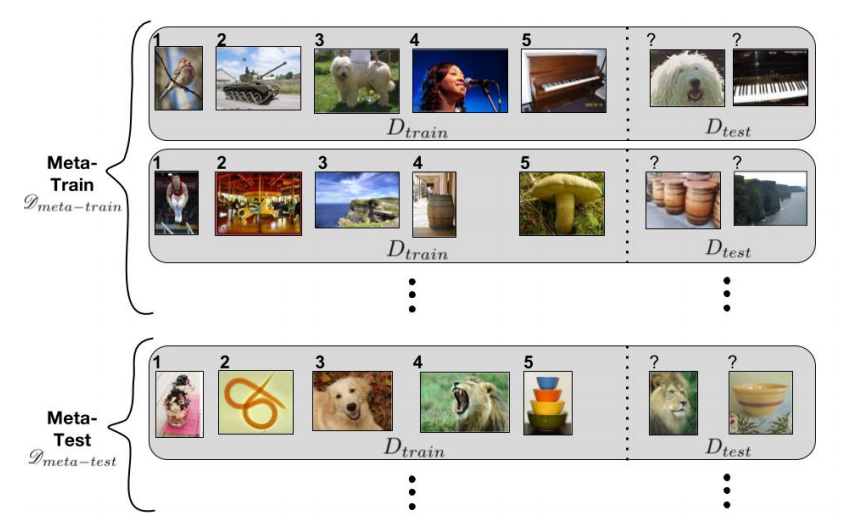
\includegraphics[width=.6\textwidth]{images/metalearning_datasets.png}

\lit{Ravi and Larochelle. 2017}
\end{center}
\smallskip

Notation: 
\begin{itemize}
	\item meta-train: $\mdata = \{(\dataset^{\text{train}}_1,\dataset^{\text{test}}_1), \ldots, \dataset^{\text{train}}_n,\dataset^{\text{test}}_n)  \}$
\end{itemize}


$\leadsto$ Assumption: At meta-test we only have a few examples ("few shots") from a similar task

\end{frame}
%-----------------------------------------------------------------------
%----------------------------------------------------------------------
\begin{frame}[c]{Optimization-based Initialization \litw{Fin et al. 2017}}

\begin{itemize}
	\item Idea: Acquire $\phi$ through optimization
	$$\argmax_{\phi_i} \log p(\dataset^{\text{train}}_i | \phi) + \log p(\phi_i | \theta)$$
	\pause
	\smallskip
	\item[$\leadsto$] Meta-parameters $\theta$ serve as a prior
	\pause
	\smallskip
	\item One successful form of prior knowledge is the initialization of DNNs for fine-tuning (at test time):
	$$ \phi \leftarrow \theta - \alpha \nabla_\theta \loss(\theta, \dataset^{\text{train}})$$
	where $\theta$ are pre-trained weights and $\dataset^{\text{train}}$ is data for a new task
	\pause
	\smallskip
	\item Meta-learning task:
	$$\argmin_{\theta} \sum_{\text{task } i} \loss(\theta - \alpha \nabla_\theta \loss(\theta, \dataset_i^{\text{train}}),  \dataset_i^{\text{test}})$$
	
\end{itemize}


\end{frame}
%-----------------------------------------------------------------------
%----------------------------------------------------------------------
\begin{frame}[c]{Model-Agnostic Meta-Learning (MAML) \litw{Fin et al. 2017}}

	$$\argmin_{\theta} \sum_{\text{task } i} \loss(\theta - \alpha \nabla_\theta \loss(\theta, \dataset_i^{\text{train}}),  \dataset_i^{\text{test}})$$


\begin{center}
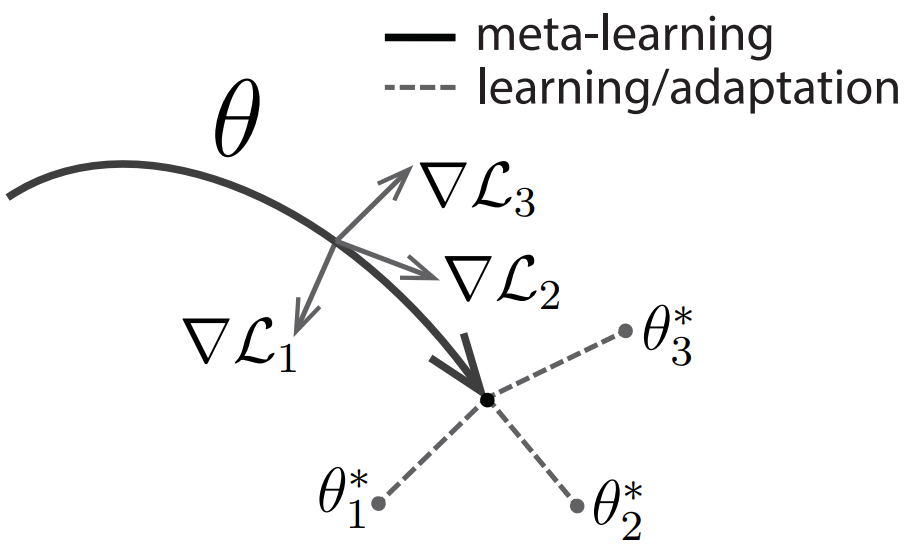
\includegraphics[width=0.6\textwidth]{images/maml.png}
\end{center}
\smallskip
where $\theta_i^*$ are the optimal weights for Task $i$

\end{frame}
%-----------------------------------------------------------------------
%----------------------------------------------------------------------
\begin{frame}[c]{MAML Algorithm \litw{Fin et al. 2017}}

\begin{algorithm}[H]
	\Input{Distribution $p(\mathcal{T})$ over tasks, learning rates $\alpha$ and $\beta$
	}
	\BlankLine
	randomly initilize $\theta$;\\
	\pause
	\While{not done}{
		Sample batch of tasks $\mathcal{T}_i \sim p(\mathcal{T})$;\\
		\pause
		\ForEach{$\mathcal{T}_i$}{
			Evaluate $\nabla_\theta \loss_{\mathcal{T}_i}(f_{\theta_i})$ with respect to K examples;\\
			\pause
			Compute adapted parameters with gradient descent:\newline $\theta_i' \rightarrow \theta_i - \alpha \nabla_\theta \loss_{\mathcal{T}_i}(f_{\theta_i})$;
			}
		\pause
		Update $\theta \rightarrow \theta - \beta \nabla_\theta \sum_{\mathcal{T}\sim p(\mathcal{T})} \loss_{\mathcal{T}_i}(f_{\theta'_i})$;
	}
	
\Return{Pre-trained weights $\theta$}
\end{algorithm}

\end{frame}
%-----------------------------------------------------------------------
%----------------------------------------------------------------------
\begin{frame}[c]{MAML Algorithm for Supervised Learning\litw{Fin et al. 2017}}

\begin{algorithm}[H]
	\Input{Distribution $p(\mathcal{T})$ over tasks, learning rates $\alpha$ and $\beta$
	}
	\BlankLine
	randomly initilize $\theta$;\\
	\While{not done}{
		Sample batch of tasks $\mathcal{T}_i \sim p(\mathcal{T})$;\\
		\ForEach{$\mathcal{T}_i$}{
			\alert{Sample $K$ datapoints $\dataset = \{x^{(j)}, y^{(j)} \}$ from $\mathcal{T}_i$;}\\
			Evaluate $\nabla_\theta \loss_{\mathcal{T}_i}(f_{\theta_i})$ \alert{using $\dataset$ and $ \loss_{\mathcal{T}_i}$};\\
			Compute adapted parameters with gradient descent:\newline $\theta_i' \rightarrow \theta_i - \alpha \nabla_\theta \loss_{\mathcal{T}_i}(f_{\theta_i})$;\\
			\alert{Sample datapoints $\dataset' = \{x^{(j)}, y^{(j)}\}$ from $\mathcal{T}_i$ for the meta-update;}
		}
		Update $\theta \rightarrow \theta - \beta \nabla_\theta \sum_{\mathcal{T}\sim p(\mathcal{T})} \loss_{\mathcal{T}_i}(f_{\theta'_i})$ using each \alert{$\dataset'$ and $\loss_{\mathcal{T}_i}$};
	}
	
	\Return{Pre-trained weights $\theta$}
\end{algorithm}

\end{frame}
%-----------------------------------------------------------------------
%----------------------------------------------------------------------
\begin{frame}[c]{Discussion of MAML}

\begin{itemize}
	\item MAML can improve the performance on \alert{few-short learning task}\\
	(i.e., we only have few examples for each task)\\
	where we use only a \alert{few update steps}
	\pause
	\smallskip
	\item MAML uses \alert{second-order derivatives} which makes it only applicable to small datasets\\
	\begin{itemize}
		\item first-order approximation of MAML can also perform quite well
	\end{itemize}
	\pause
	\smallskip
	\item MAML-fine-tuning requires \alert{backpropagation through the entire network}
	\begin{itemize}
		\item in "traditional" fine-tuning, we only fine-tune the last layer(s)
	\end{itemize}
	
\end{itemize}

\end{frame}
%-----------------------------------------------------------------------
%-----------------------------------------------------------------------
\section{Learning to Learn \& Optimize}
%----------------------------------------------------------------------
\begin{frame}[c]{Learning to Learn}

\begin{block}{Idea}
	\begin{itemize}
		\item Learn algorithms directly, i.e., how to search in the solution space
		\item First idea: learn weight updates of a neural network
	\end{itemize}
\end{block}

\pause

\begin{block}{Learning to learn by gradient descent by gradient descent\newline \litw{Andrychowicz et al'16}}
	Weight updates (note: \alert{$\theta$ denote DNN weights!}):
	\begin{equation}
	\theta_{t+1} = \theta_t - \alpha_t \nabla f(\theta_t) \nonumber
	\end{equation}
	\pause
	Even more general:
	\begin{equation}
	\theta_{t+1} = \theta_t + g_t(\nabla f(\theta_t), \phi) \nonumber
	\end{equation}
	where $g$ is the optimizer and $\phi$ are the parameters of the optimizer $g$.\\
	\pause
	$\leadsto$ \alert{Goal: Optimize $f$ wrt $\theta$ by learning $g$}
\end{block}

\end{frame}
%----------------------------------------------------------------------
%----------------------------------------------------------------------
\begin{frame}[c]{Learning to Learn: Objective \litw{Andrychowicz et al'16}}

\vspace{-0.5cm}
\begin{equation}
\mathcal{L}(\phi) = \mathbb{E}\left[ f(\theta^*(f,\phi)) \right]\nonumber
\end{equation}

where $\mathcal{L}$ is a loss function and $\theta^*(f,\phi)$ are the optimized weights $\theta^*$ by using the optimizer parameterized with $\phi$ on function $f$.

\pause

%\vspace{-0.5cm}
\begin{equation}
\mathcal{L}(\phi) = \mathbb{E}\left[\sum_{t=1}^T w_t f(\theta_t)\right]\nonumber
\end{equation}

\pause
where $w_t$ are arbitrary weights associated with each time step
and 

\pause
\vspace{-0.5cm}
\begin{eqnarray}
\theta_{t+1} = \theta_t + g_t\\\nonumber
\begin{pmatrix}g_t\\h_{t+1}\end{pmatrix} = m(\nabla_\theta f(\theta_t), h_t, \phi)\nonumber
\end{eqnarray}

\pause
$\leadsto$ Goal: Learn $m$ via $\phi$ by using gradient descent by optimizing $\mathcal{L}$ \\
\pause
$\leadsto$ ``Learning to learn gradient descent by gradient descent''
\end{frame}
%----------------------------------------------------------------------
%----------------------------------------------------------------------
\begin{frame}[c]{Learning to Learn: LSTM approach \litw{Andrychowicz et al'16}}

\begin{description}
\item[Optimizee] Target network to be trained
\item[Optimizer] LSTM with hidden state $h_t$ that predicts weight updates $g_t$
\end{description}

\medskip

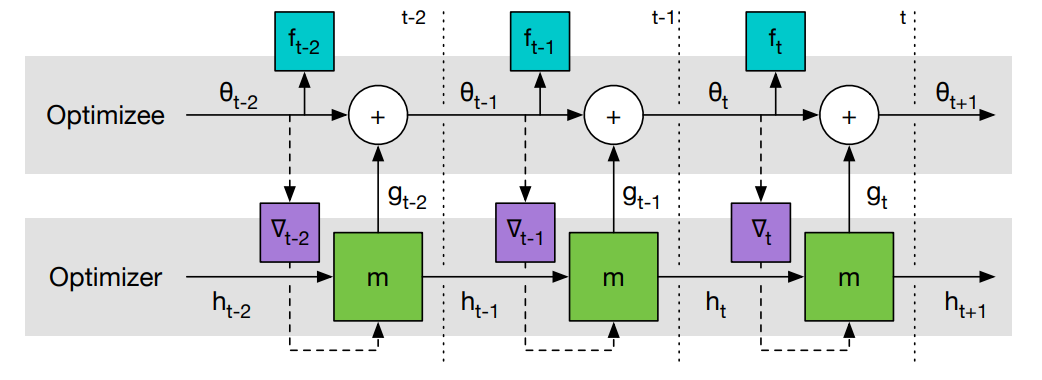
\includegraphics[width=1\textwidth]{images/learning_to_learn_lstm}

\end{frame}
%----------------------------------------------------------------------
%----------------------------------------------------------------------
\begin{frame}[c]{Learning to Learn with LSTM: Results \litw{Andrychowicz et al'16}}

\centering
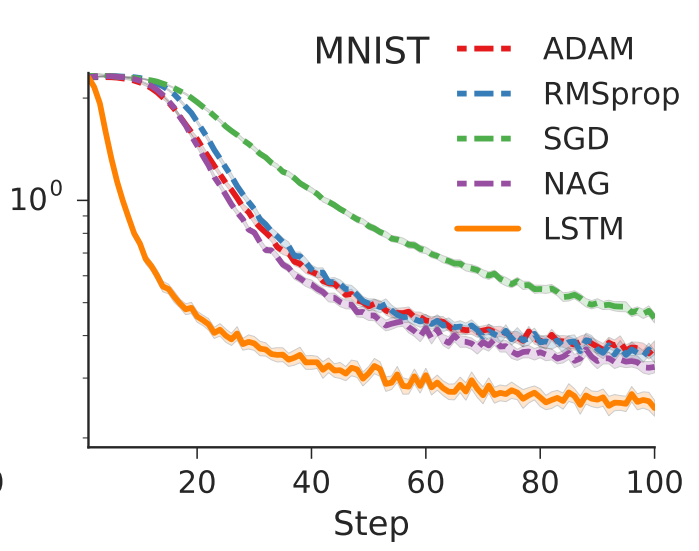
\includegraphics[width=0.7\textwidth]{images/l2l_mnist_base}

\end{frame}
%----------------------------------------------------------------------
%----------------------------------------------------------------------
\begin{frame}[c]{Learning to Learn with LSTM: Results \litw{Andrychowicz et al'16}}

Changing the original architecture of the DNN:
\smallskip

\centering
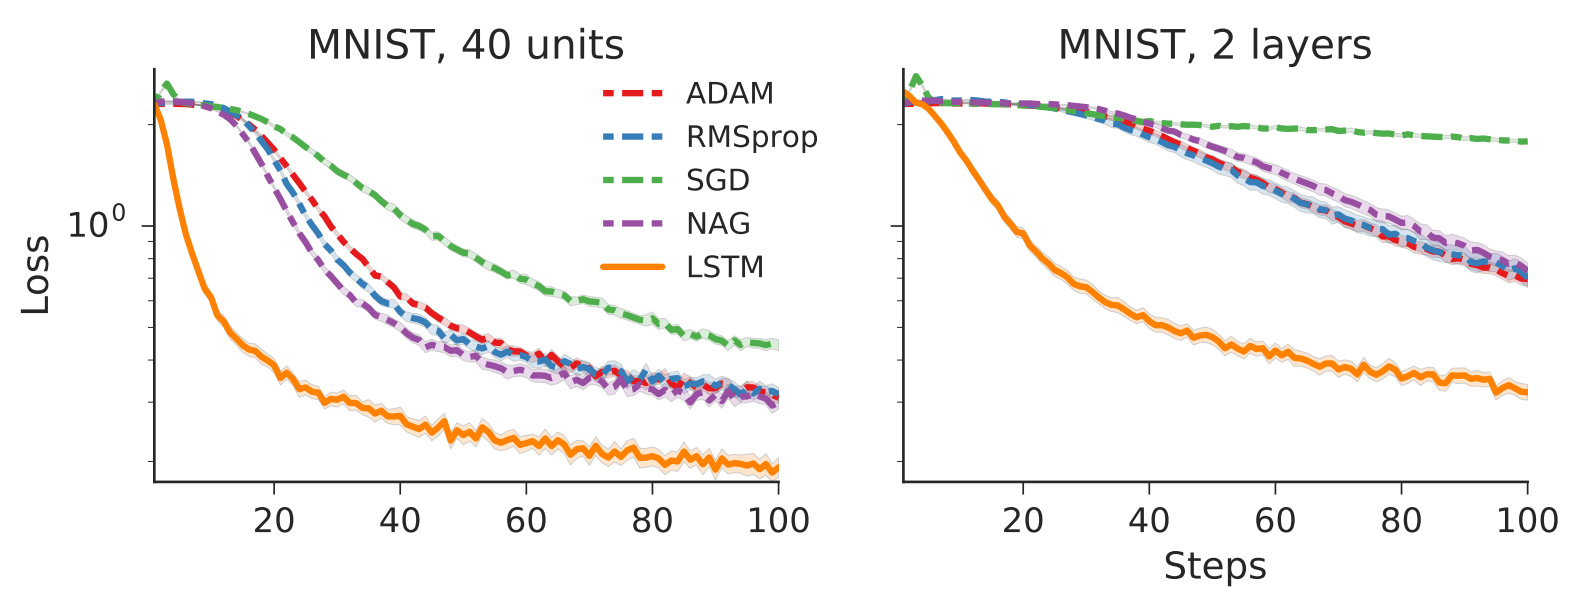
\includegraphics[width=0.9\textwidth]{images/l2l_mnist_okchange}

$\leadsto$ learnt optimizer is robust against some architectural changes

\pause
\smallskip
How can we learn the weight updates for larger networks? \hands

\end{frame}
%----------------------------------------------------------------------
%----------------------------------------------------------------------
\begin{frame}[c]{Learning to Learn with LSTM: Results\newline \litw{Andrychowicz et al'16}}

Changing the activation function to ReLU:
\smallskip

\centering
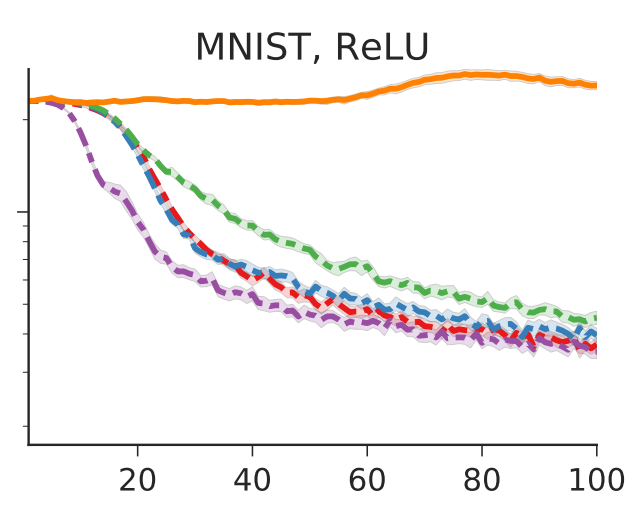
\includegraphics[width=0.6\textwidth]{images/l2l_mnist_relu}

$\leadsto$ fails on other activation functions

\end{frame}
%----------------------------------------------------------------------
%----------------------------------------------------------------------
\begin{frame}[c]{Learning Step Size Controllers \litw{Daniel et al'16}}

\begin{itemize}
	\item \alert{Idea:} Learn the hyperparameters of the weight update 
\end{itemize}

\begin{equation}
\theta_{t+1} = \theta_t - \alpha_t \nabla f(\theta_t) \nonumber
\end{equation}

\begin{itemize}
	\item For SGD, this would be for example the learning rate $\alpha$
	\pause
	\item \alert{Note}: $\alpha$ have to be adapted in the course of the training
	\begin{itemize}
		\item similar to learning rate schedules (e.g., cosine annealing)
	\end{itemize}
	\pause
	\item \alert{Note(ii)}: later we denote the learnt hyperparameters as $\lambda$
	\medskip
	\pause
	\item \alert{Idea:} Use reinforcement learning to learn a policy $\pi: s \mapsto a$ to control the learning rate (or other adaptive hyperparameters)
\end{itemize}



\end{frame}
%----------------------------------------------------------------------
%----------------------------------------------------------------------
\begin{frame}[c]{Recap: Reinforcement Learning \litw{Barto \& Sutton; RL Book}}

\begin{center}
	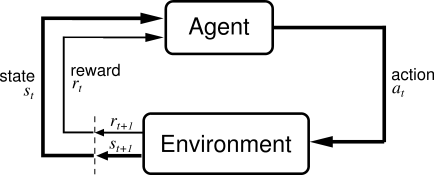
\includegraphics[width=0.6\textwidth]{images/suttonbarto_rl.png}
\end{center}

\pause

\begin{eqnarray}
\pi^* \argmax_{\pi} \mathbb{E}_{\pi} \left[ \sum^{T}_{t=1} \gamma^{t-1} r_t \mid s_0 \right] \nonumber
\end{eqnarray}

The goal is to find the optimal policy $\pi^{*}: s \mapsto a$ starting in a state $s_0$\\ (or in expectation of $s_0$) s.t. following $\pi^{*}$ from $s$ maximizes the expected (discounted) reward~$R$.


\end{frame}
%----------------------------------------------------------------------
%----------------------------------------------------------------------
\begin{frame}[c]{RL for Step Size Controllers: State \litw{Daniel et al'16}}

\textbf{Predictive change in function value:}

$$s_1 = \log \left( \text{Var}(\Delta \tilde{f}_i ) \right)$$
$$\Delta \tilde{f}_i = \tilde{f}(x_i; \theta + \delta \theta) - f(x_i; \theta)$$

where $\tilde{f}(x_i; \theta + \delta \theta)$ is done by a first order Taylor expansion

\pause
\textbf{Disagreement of function values:}
$$ s_2 = \log \left(\text{Var}(f(x_i; \theta)) \right)$$

\pause

\textbf{Discounted Average} (smoothing noise from mini-batches):
$$\hat{s}_i \leftarrow \gamma \hat{s_i} + (1 - \gamma) s_i$$

\pause

\textbf{Uncertainty Estimate}:
$$s_{K+i} \leftarrow \gamma s_{K+i} + (1-\gamma) (s_i - \hat{s}_i)^2$$


\end{frame}
%----------------------------------------------------------------------
%----------------------------------------------------------------------
\begin{frame}[c]{RL for Step Size Controllers: Learning \litw{Daniel et al'16}}

Reward (average loss improvement over time):

$$r = \frac{1}{T-1} \sum_{t=2}^T \left(\log(\loss_{t-1}) - \log(\loss_t)\right)$$

\pause

Optimal Policy:

$$\pi^*(\lambda \mid s) \in \argmax_{\pi} \int \int p(s) \pi(\lambda\mid s)r(\lambda,s) \texttt{d}s \texttt{d}\lambda $$

\pause

The policy $\pi$ is learnt as a controller $\lambda = g(s, \phi)$; leading to

$$\pi^*(\phi) \in \argmax_{\pi} \int \int p(s) \pi(\phi)r(g(s;\phi),s) \texttt{d}s \texttt{d}\lambda $$

\pause

\begin{itemize}
	\item can be learnt for example via Relative Entropy Policy Search (REPS) \lit{Peter et al. 2010}
\end{itemize}

\end{frame}
%----------------------------------------------------------------------
%----------------------------------------------------------------------
\begin{frame}[c]{RL for Step Size Controllers: Training \litw{Daniel et al'16}}

\begin{itemize}
	\item We want to obtain robust policies, i.e., good performance for many different DNN architectures
	\begin{itemize}
		\item[$\leadsto$] Sample architectures e.g., with different numbers of filters and layers
		\item[$\leadsto$] (Sub-)Sample dataset
		\item[$\leadsto$] Sample number of optimization steps
	\end{itemize}
\end{itemize}

\centering
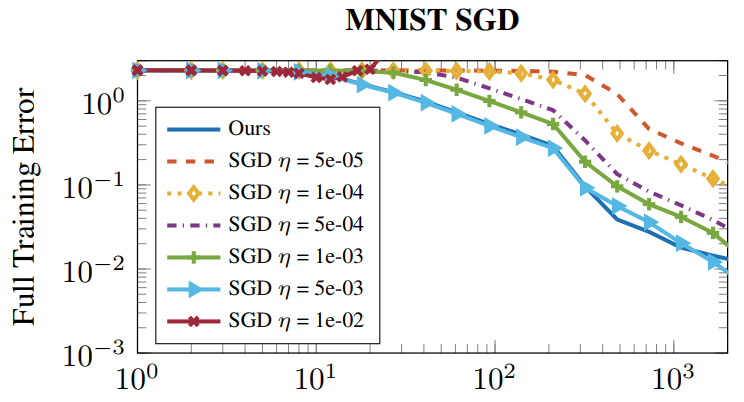
\includegraphics[width=0.6\textwidth]{images/l2stepsizecontroler_mnist_training.png}

\end{frame}
%----------------------------------------------------------------------
%----------------------------------------------------------------------
\begin{frame}[c]{Learning Black-box Optimization~\litw{Chen et al'17}}

\begin{block}{Black Box Optimization Setting}
\begin{enumerate}
\item Given the current state of knowledge $h_t$ propose a query point $x_t$
\item Observe the response $y_t$
\item Update any internal statistics to produce $h_{t+1}$
\end{enumerate}
\end{block}

\pause

\begin{block}{Learning Black Box Optimization}
Essentially, same idea as before:
\begin{eqnarray}
h_t, x_t = \text{RNN}_\phi(h_{t-1}, x_{t-1}, y_{t-1}) \nonumber \\
y_t \sim p(y|x_t)\nonumber
\end{eqnarray}

\begin{itemize}
\item Using recurrent neural network (RNN) to predict next $x_t$.
\item $h_t$ is the internal hidden state 
\pause
\item \alert{Remark:} in a black-box setting, we don't have gradient information!
\end{itemize}

\end{block}



\end{frame}
%----------------------------------------------------------------------
%----------------------------------------------------------------------
\begin{frame}[c]{Learning Black-box Optimization: Loss Functions\newline \litw{Chen et al'17}}

\begin{itemize}
\item Sum loss: Provides more information than final loss
\end{itemize}
\begin{equation}
\mathcal{L}_{\text{sum}}(\phi) = \mathbb{E}_{f,y_{1:T-1}}\left[\sum_{t=1}^T f(x_t)\right]\nonumber
\end{equation}

\pause

\begin{itemize}
\item EI loss: Try to learn behavior of Bayesian optimizer based on expected improvement (EI)
\begin{itemize}
\item requires model (e.g., GP)
\end{itemize}
\end{itemize}
\begin{equation}
\mathcal{L}_{\text{EI}}(\phi) = - \mathbb{E}_{f,y_{1:T-1}}\left[\sum_{t=1}^T \text{EI}(x_t | y_{1:t-1})\right]\nonumber
\end{equation}

\pause

\begin{itemize}
\item Observed Improvement Loss:
\end{itemize}

\begin{equation}
\mathcal{L}_{\text{OI}}(\phi) = \mathbb{E}_{f,y_{1:T-1}}\left[\sum_{t=1}^T \min \left\{f(x_t) - \min_{i<t}(f(x_i)),0 \right\}  \right]\nonumber
\end{equation}

\end{frame}
%----------------------------------------------------------------------
%----------------------------------------------------------------------
\begin{frame}[c]{Learning Black-box Optimization: Results\newline \litw{Chen et al'17}}

\centering
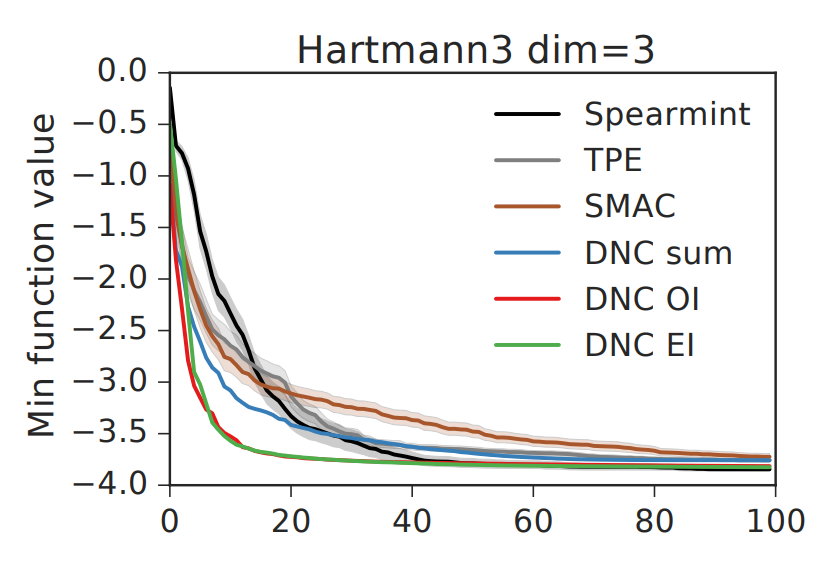
\includegraphics[width=0.6\textwidth]{images/l2bo_hartmann3}

\begin{itemize}
\item Hartmann3 is an artifical function with 3 dimensions
\pause
\item[$\leadsto$] $\mathcal{L}_{\text{OI}}$ and $\mathcal{L}_{\text{EI}}$ perform best
\item[$\leadsto$] $\mathcal{L}_{\text{OI}}$ easier to compute than $\mathcal{L}_{\text{EI}}$\\ because we need a predictive model to compute EI 
\end{itemize}

\end{frame}
%----------------------------------------------------------------------
%----------------------------------------------------------------------
\begin{frame}[c]{Learning to Optimize via Reinforcement Learning\newline \litw{Li and Malik'17}}

\centering
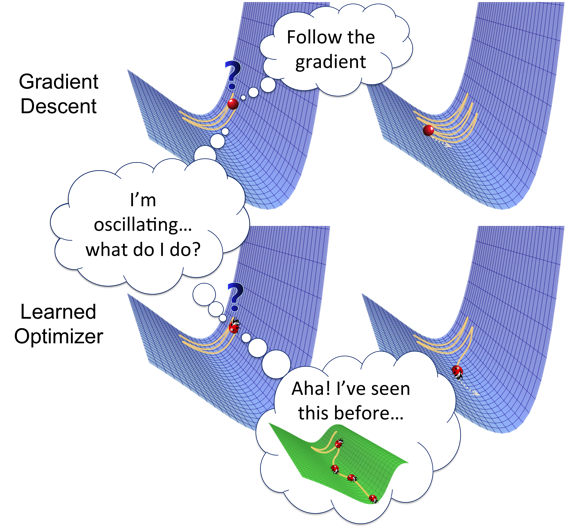
\includegraphics[width=0.6\textwidth]{images/l2o_comic}

\tiny
Source: \url{https://bair.berkeley.edu/blog/2017/09/12/learning-to-optimize-with-rl/}

\end{frame}
%----------------------------------------------------------------------
%----------------------------------------------------------------------
\begin{frame}[c]{Learning to Optimize via Reinforcement Learning\newline \litw{Li and Malik'17}}

\begin{block}{Reinforcement Learning for Learning to Optimize}
\begin{description}
\item[State] current location, objective values and gradients evaluated at the current and past locations
\pause
\item[Action] Step update $\Delta x$
\pause
\item[Transition] $x_t \leftarrow x_{t-1} + \Delta x$
\pause
\item[Cost/Reward] Objective value at the current location
\begin{itemize}
\item Since the RL agent will optimize the cumulative cost, this is equivalent to $\mathcal{L}_{\text{sum}}$
\item encourages the policy to reach the minimum of the objective function as quickly as possible
\end{itemize}
\pause
\item[Policy] DNN predicting $\mu_d$ of Gaussian (with constant variance $\sigma^2$)\\ for dimension $d$; sample $\Delta x_d \sim \mathcal{N}(\mu_d, \sigma^2)$
\pause
\item[Training Set] randomly generated objective functions
\end{description}
\end{block}

\end{frame}
%----------------------------------------------------------------------
%----------------------------------------------------------------------
\begin{frame}[c]{Learning to Optimize via Reinforcement Learning\newline Results \litw{Li and Malik'17}}

\centering
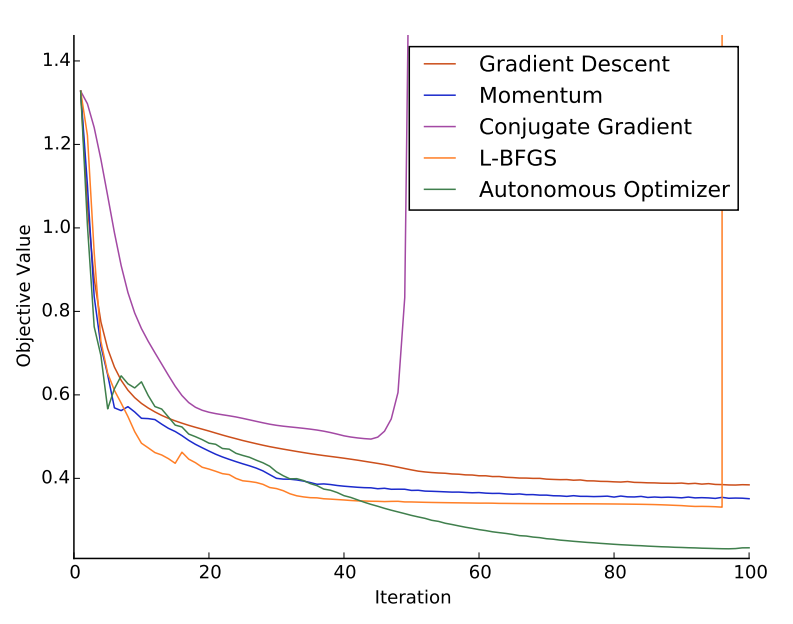
\includegraphics[width=0.5\textwidth]{images/l2o_dnn}

\begin{itemize}
\item 2-layer DNN with ReLUs
\item Training datasets for training RL agent:\\ four multivariate Gaussians and sampling 25 points from each
\begin{itemize}
\item[$\leadsto$] hard toy problem
\end{itemize}
\end{itemize}

\end{frame}
%----------------------------------------------------------------------
%----------------------------------------------------------------------
\begin{frame}[c, fragile]{Learning Acquisition Functions\newline Results \litw{Volpp et al.'19}}

\begin{itemize}
	\item Instead of learning everything, it might be sufficient to \alert{learn hand-design heuristics}
	\item In Bayesian Optimization (BO), the most critical hand-design heuristic is the acquisition function
	\begin{itemize}
		\item trade-off between exploitation and exploration
		\item Depending on the problem at hand, you might need a different acquisition function
		\item Choices:
		\begin{itemize}
			\item probability of improvement (PI)
			\item expected improvement (EI)
			\item upper confidence bounds (UCB)
			\item entropy search (ES) -- quite expensive!
			\item knowledge gradient (KG)
			\item ...
		\end{itemize} 
	\end{itemize}
	\item \alert{Idea:} Learn a \emph{neural acquisition function} from data
\end{itemize}

$\leadsto$ Replace acquisition function 

\end{frame}
%----------------------------------------------------------------------
%-----------------------------------------------------------------------
\begin{frame}[c,fragile]{Bayesian Optimization: Algorithm}

\begin{algorithm}[H]
	\Input{Search Space $\mathcal{X}$,
		black box function $f$, 
		\alert{acquisition function $\alpha$,}
		maximal number of function evaluations $m$
	}
	\BlankLine
	$\mathcal{D}_0$ $\leftarrow$ initial\_design($\mathcal{X}$); \\
	\For{n = $1, 2, \ldots m - |D_0|$}{
		$\surro: \conf \mapsto y$ $\leftarrow$ fit predictive model on $\mathcal{D}_{n-1}$;\\
		select $x_{n}$ by optimizing $x_{n} \in \argmax_{x \in \mathcal{X}} \alert{\alpha(x; \mathcal{D}_{n-1}, \surro)}$;\\
		Query $y_{n} := f(x_{n})$;\\
		Add observation to data $D_{n} := D_{n-1} \cup \{\langle x_{n}, y_{n} \rangle \}$;
	}
	\Return{Best $x$ according to $D_m$ or $\surro$}
	\caption{Bayesian Optimization (BO)}
\end{algorithm}


\end{frame}
%-----------------------------------------------------------------------
%-----------------------------------------------------------------------
\begin{frame}[c]{Neural Acquisition Function \litw{Volpp et al.'19}}

Although the acquisition function $\alpha$ depends on the history $\mathcal{D}_{n-1}$ and the predictive model $\surro$, $\alpha$ mainly makes use of the predictive mean $\mu$ and variance $\sigma^2$.

\pause
\bigskip

Neural acquisition function (AF):

\begin{eqnarray}
\alpha_\theta(x) = \alpha_\theta(\mu_t(x), \sigma_t(x)) \nonumber
\end{eqnarray}

where $\theta$ are the parameters of a neural network,\\ and $\mu$ and $sigma$ are its inputs.

\begin{itemize}
	\item Since the input is not $x$, it allows to learn scalable acquisition function
	\item No calibration of hyperparameter necessary, once the neural AF is learnt
\end{itemize}

\end{frame}
%-----------------------------------------------------------------------
%-----------------------------------------------------------------------
\begin{frame}[c]{RL to train Neural AF \litw{Volpp et al.'19}}

\begin{description}
	\item[Policy $\pi_\theta$:] Neural acquisition function $\alpha_\theta$
	\pause
	\item[Episode:] run of $\pi$ on $f\in \mathcal{F}'$
	\begin{itemize}
		\item $\mathcal{F}$ is a set of functions we can sample functions from
	\end{itemize}
	\pause
	\item[State $s_t$:] $\mu_t$ and $\sigma_t$ on a set of points $\xi_t$
	\pause
	\item[Action $a_t$:] Sampled point $x_t$
	\pause
	\item[Reward $r_t$:] negative simple regret: $r_t = f(x^*) - f(\hat{x})$
	\begin{itemize}
		\item assumes that we can estimate the optimal $x^*$ for \emph{training} functions
	\end{itemize}
	\pause
	\item[Transition probability]: Noisy evaluation of $f$ and the predictive model update
\end{description}

\end{frame}
%-----------------------------------------------------------------------
%-----------------------------------------------------------------------
\begin{frame}[c]{State \litw{Volpp et al.'19}}

\begin{itemize}
	\item The state is described by a discrete set of points $\xi_t = \{\xi_n\}^N_{n=1}$
	\pause
	\item We feed these points through the predictive model and the neural AF to obtain $\alpha_\theta(\xi_i) = \alpha_\theta(\mu_t(\xi_i), \sigma_t(\xi_i)) $
	\pause
	\item $\alpha_\theta(\xi_i)$ are interpreted as the logits of multinomial distribution, s.t.
	$$\pi_\alpha(\cdot \mid s_t) = \text{Mult}\left[\alpha_\theta(\xi_1), \ldots, \alpha_\theta(\xi_N) \right] $$
	\pause
	\item Due to curse of dimensionality, we need a two step approach for~$\xi_t$
	\begin{enumerate}
		\item sample $\xi_{\text{global}}$ using a coarse Sobol grid
		\item sample $\xi_{\text{local}}$ using local optimization starting from the best samples in $\xi_{\text{global}}$
	\end{enumerate}
	\item[$\leadsto$] $\xi_t = \xi_{\text{global}} \cup \xi_{\text{lokal}}$ 
\end{itemize}

\end{frame}
%-----------------------------------------------------------------------
%-----------------------------------------------------------------------
\begin{frame}[c,fragile]{Learning Acquisition Functions\newline Results \litw{Volpp et al.'19}}

\centering
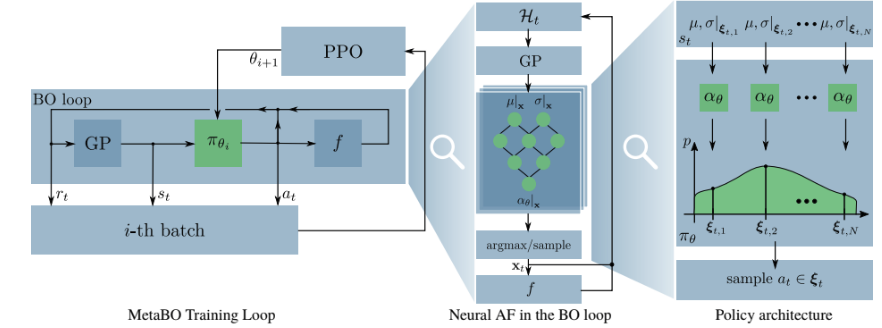
\includegraphics[width=1.0\textwidth]{images/l2acq.png}


\end{frame}
%-----------------------------------------------------------------------
%-----------------------------------------------------------------------
\begin{frame}[c]{Results on Artificial Functions \litw{Volpp et al.'19}}

\centering
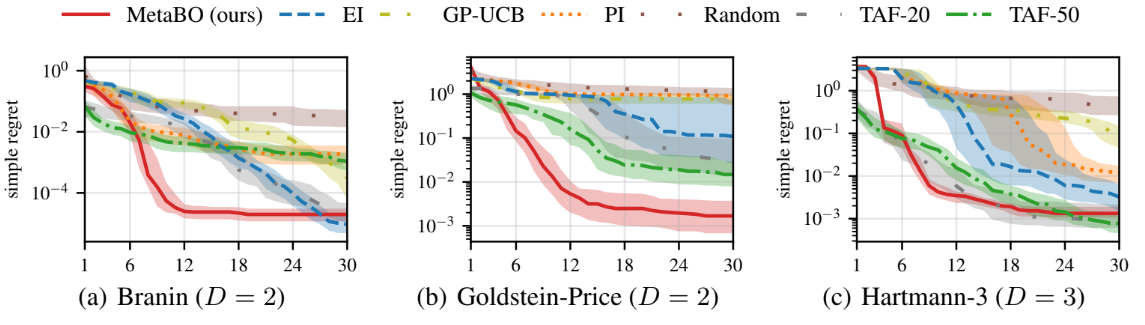
\includegraphics[width=1.0\textwidth]{images/l2acq_results.png}

\medskip

\begin{itemize}
	\item Approach by \lit{Volpp et al. '19} called MetaBO
	\item MetaBO performs better than other acquisition functions (EI, GP-UBC, PI) and other baselines (Random, TAF)
\end{itemize}

\pause

\alert{Assumption}: You have a family of functions at hand that resembles your target functions.

\end{frame}
%-----------------------------------------------------------------------

%----------------------------------------------------------------------
\begin{frame}[c]{Learning Goals}

After these lectures, you are able to \ldots

\begin{itemize}
	\item explain the \alert{high-level principles of meta-learning} and its facets
	\item use \alert{algorithm selection} to predict the best algorithm for a dataset
	\item improve the performance of AutoML tools by \alert{warmstarting its search}
	\item \alert{transfer knowledge} between DNNs by determining initial weights
	\item \alert{learn} a DNN which can \alert{train} another DNNs
	\item \alert{learn} a policy \alert{to optimize} a black-box function
	\item \alert{learn} policies to either \alert{replace} algorithm components\\ or to \alert{control} hyperparameters
\end{itemize}

\end{frame}
%-----------------------------------------------------------------------

%----------------------------------------------------------------------
\begin{frame}[c]{Literature [These are links]}

\begin{itemize}
	\item \lit{\href{https://arxiv.org/abs/1811.11597}{Automated Algorithm Selection: Survey and Perspectives}}	
	\item \lit{\href{https://arxiv.org/abs/1703.03400}{MAML: Model-Agnostic Meta-Learning for Fast Adaptation of Deep Networks}}	
	\item \lit{\href{https://ml.informatik.uni-freiburg.de/papers/15-NIPS-auto-sklearn-preprint.pdf}{Efficient and Robust Automated Machine Learning}}	
	\item \lit{\href{https://arxiv.org/abs/1606.04474}{Learning to learn by gradient descent by gradient descent}}	
	\item \lit{\href{https://arxiv.org/abs/1611.03824}{Learning to Learn without Gradient Descent by Gradient Descent}}	
	\item \lit{\href{https://arxiv.org/abs/1606.01885}{Learning to Optimize}}	
	\item \lit{\href{https://arxiv.org/abs/1904.02642}{Meta-Learning Acquisition Functions for Bayesian Optimization}}	
\end{itemize}

\end{frame}
%----------------------------------------------------------------------


